\chapter{Redakcja pracy dyplomowej}
\label{chap:trzeci}



%-------------------------------------------------------
\section{Parametry dokumentu}
Osoby korzystające z narzędzia do składu tekstu \LaTeX~ i opracowanego szablonu, nie muszą martwić się formatowaniem dokumentu. Wszelkie niezbędne ustawienia zostały już zawarte w szablonie. W takim wypadku można skoncentrować się przede wszystkim na stronie merytorycznej pracy.

W przypadku użycia innych narzędzi (np. edytora tekstu Microsoft Word), konieczne jest prawidłowe zdefiniowanie parametrów tworzonego dokumentu. Powinien on być wizualnie zgodny z niniejszym ,,przewodnikiem dyplomanta'', który został przygotowany przy użyciu opracowanego szablonu. Rozmiar strony należy ustalić zgodnie z formatem A4, a wielkość marginesów: na 30mm (lewy), 20mm (prawy), 25mm (górny) oraz 25mm (dolny). Wcięcia akapitowe 12.5mm. Wielkość tekstu zasadniczego (\textit {Times New Roman}) powinna wynosić 12 punktów, natomiast odstępy między wierszami (interlinia) posiadać wartość 1,5.

Utworzony dokument (plik) powinien posiadać nazwę zawierającą: (1) nazwisko oraz pierwsza litera imienia dyplomanta, (2) tytuł pracy (lub istotny fragment), (3) numer wersji pliku. Przykładowa nazwa drugiej wersji dokumentu Jana Nowaka:\\

\textbf{NowakJ-Ekonomiczne uwarunkowania rozwoju zawodowego-v2
}

%-------------------------------------------------------
\section{Strona tytułowa}
Strona tytułowa pracy dyplomowej powinna być zgodna ze stroną tytułową ,,przewodnika dyplomanta'' i powinna zawierać: (1) nazwę uniwersytetu oraz instytutu, (2) kierunek i specjalność studiów, (3) imię i nazwisko studenta oraz nr jego albumu, (4) rodzaj pracy dyplomowej, (5) imię i nazwisko promotora, (6) miejscowość oraz rok sporządzenia pracy.


%-------------------------------------------------------
\section{Spis treści}
Spis treści należy umieścić na początku dokumentu, po stronie tytułowej pracy. Powinien on zawierać wykaz rozdziałów oraz głównych składowych rozdziałów, wraz z podaną numeracją stron. Należy wzorować się na spisie treści znajdującym się w ,,przewodniku dyplomanta''.


%-------------------------------------------------------
\section{Tekst zasadniczy pracy}

Zasadniczy tekst pracy składa się z paragrafów o strukturze zaprezentowanej przez \citet{website:paragraph}. Pożądane jest, aby każdy paragraf składał się z co najmniej kilku zdań. Należy unikać długich zdań, wielokrotnie złożonych. W treści pracy dyplomowej należy używać wyłącznie języka formalnego, stosując typowe w takich opracowaniach wyrażenia i zwroty \citep{website:zimny, weglinska}. Zgodnie z polskim piśmiennictwem należy unikać stosowania formy osobowej.

Należytej uwagi wymaga także stosowanie skrótów. Każde pierwsze wystąpienie skrótu w dokumencie powinno zostać uzupełnione pełnym jego objaśnieniem, podanym w nawiasie, np. UEK (Uniwersytet Ekonomiczny w Krakowie). Kolejne użycia skrótu w dokumencie nie wymagają już podawania jego rozwinięcia.

Należy również zwrócić uwagę na stosowanie pogrubionej oraz pochylonej odmiany pisma. Tę pierwszą należy stosować przede wszystkim dla wyróżnienia tytułów rozdziałów oraz podrozdziałów. Natomiast pochylenie używane jest dla wyróżnienia terminów obcojęzycznych oraz w bibliografii dla wyróżnienia tytułów opracowań i artykułów. 

Pracę nad tekstem należy bezwzględnie zakończyć jego sprawdzeniem. Konieczna jest weryfikacja jego poprawności językowej, zarówno gramatycznej, jak i stylistycznej oraz interpunkcji.


%-------------------------------------------------------
\section{Lista wypunktowana}

W przypadku użycia takiej listy w redagowanym dokumencie należy kierować się poniższymi zasadami:

\begin{itemize}
	\item zdanie poprzedzające listę wypunktowaną powinno zostać zakończone znakiem dwukropka,
	\item każdy punkt listy powinien rozpoczynać się z małej litery,
	\item na końcu każdego punktu listy należy umieścić przecinek, natomiast ostatni punkt powinien zostać zakończony kropką.
\end{itemize}

Należy również zaznaczyć, iż lista wypunktowana nie powinna stanowić zakończenia rozdziału czy podrozdziału pracy.



%-------------------------------------------------------
\section{Lista numerowana}

W przypadku użycia takiej listy w redagowanym dokumencie należy kierować się poniższymi zasadami:

\begin{enumerate}
	\item Zdanie poprzedzające listę numerowaną powinno zostać zakończone znakiem dwukropka.
	\item Każdy punkt listy numerowanej powinien rozpoczynać się z wielkiej litery.
	\item Na końcu każdego punktu listy należy umieścić znak kropki.
\end{enumerate}

Należy również zaznaczyć, iż lista numerowana nie powinna stanowić zakończenia rozdziału czy podrozdziału pracy.


%-------------------------------------------------------
\section{Rysunki}

Każdy rysunek powinien posiadać tytuł, kolejny numer oraz źródło jego pochodzenia. Jednocześnie każdy rysunek należy przywołać w tekście pracy posługując się jego numerem. Pierwsze przywołanie musi wystąpić przed pojawieniem się rysunku w dokumencie, przy czym rysunek nie musi występować bezpośrednio po tym przywołaniu, np. (...) z danych przedstawionych na rysunku \ref{fig:inflacja} wynika, iż w Polsce zaobserwować można powolny wzrost inflacji począwszy od drugiego półrocza 2019 roku (...).

\begin{figure}[ht]
	\centering
	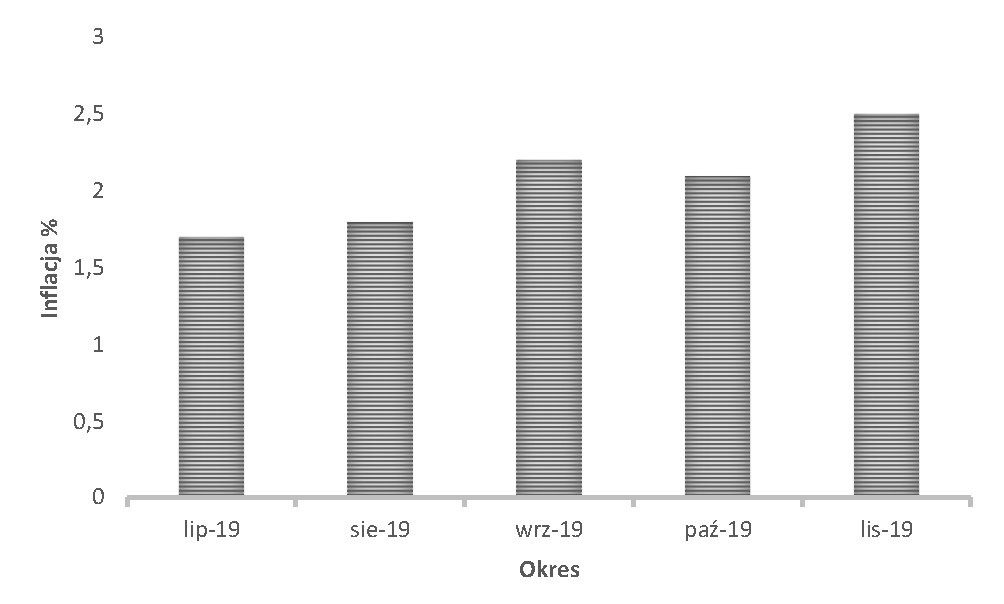
\includegraphics[width=120mm]{images/inflacja.pdf}
	\caption{Inflacja w Polsce}
	\caption*{Źródło: opracowanie własne na podstawie: \citep{barczak-brezinski}.}
	\label{fig:inflacja}
\end{figure}

Wszystkie rysunki występujące w pracy dyplomowej powinny zostać sformatowanie w jednolity sposób i wyśrodkowane. Tytuł należy umieścić pod rysunkiem, a poniżej rysunku bezwzględnie podać źródło jego.

W przywołaniach należy bezwzględnie stosować numer rysunku -- nie powinno używać się sformułowań ,,powyżej/poniżej''. Bardzo istotna jest również jakość użytych ilustracji. Najlepiej, aby rysunki zostały sporządzone samodzielnie przez autora pracy i zapisane w formacie grafiki wektorowej (EPS) (zobacz rys. \ref{fig:sinusoida}) lub jako dobrej jakości grafika rastrowa (PNG, JPG). Należy unikać umieszczania w pracy kopii rysunków (skanów) o wątpliwej jakości, zaczerpniętych z innych źródeł. Rzutuje to na ostateczną ocenę pracy. Ważne jest również zachowanie spójnej kolorystyki dla wszystkich rysunków wykorzystanych w pracy.

\begin{figure}[ht]
	\centering
	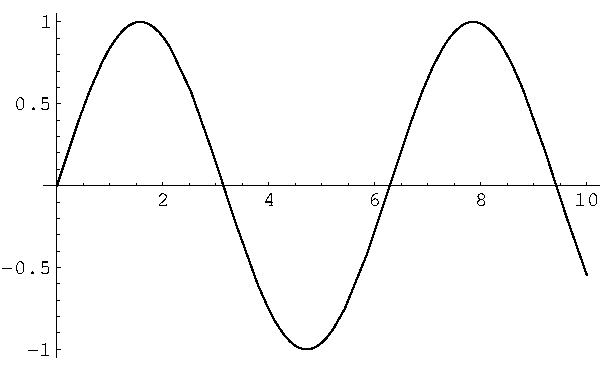
\includegraphics[width=100mm]{images/mathematica.pdf}
	\caption{Wykres funkcji}
	\caption*{Źródło: opracowanie własne.}
	\label{fig:sinusoida}
\end{figure}

Na końcu pracy należy umieścić wykaz (spis) występujących w pracy rysunków uporządkowany wg kolejności ich występowania w dokumencie.



%-------------------------------------------------------
\section{Tabele}

Każda tabela powinna posiadać tytuł, kolejny numer oraz źródło pochodzenia danych. Jeśli to możliwe, powinno się unikać dzielenia tabel -- należy umieszczać je w całości na jednej stronie. Każdą tabelę należy przywołać w tekście pracy posługując się jej numerem. Pierwsze przywołanie powinno wystąpić przed pojawieniem się tabeli w dokumencie, przy czym tabela nie musi występować bezpośrednio po tym przywołaniu, czy na tej samej stronie, np. (...) rezerwaty i pomniki przyrody wymienione w tabeli \ref{tab:rezerwaty} zlokalizowane są w pobliżu Krakowa (...).


\begin{table}[ht]
	\centering
	\caption{Rezerwaty i pomniki przyrody}
	\begin{tabularx}{\textwidth}{l c X}
		\hline
		\textbf{Nazwa rezerwatu} & \textbf{Powierzchnia}	& \textbf{Przedmiot ochrony}\\
		\hline
		Bielańskie Skałki		& 1,73 ha		& spontaniczne procesy sukcesji
												  biocenoz leśnych na skalistym,
												  dawniej pozbawionym lasu terenie\\
		Bonarka					& 2,29 ha		& rezerwat geologiczny, uskoki
												  geologiczno-tektoniczne,
												  powierzchnie abrazyjne,
												  odsłonięte utwory jurajskie,
												  kredowe i trzeciorzędowe\\
		Panieńskie Skały		& 6,41 ha		& wąwóz jurajski z wychodniami skał
												  wapiennych, naturalny las bukowy i grądowy\\
		Skałki Przegorzalskie	& 1,38 ha		& skała z roślinnością kserotermiczną\\
		Skołczanka				& 36,77 ha		& zrębowe wzgórze wapienne ze zróżnicowanymi
												  biocenozami, stanowisko fauny środowisk
												  kserotermicznych, w tym rzadkich
												  i zagrożonych gatunków owadów\\
		\hline		
	\end{tabularx}
	\caption*{Źródło: opracowane na podstawie: \citep{alexandrowicz1975katalog}.}
	\label{tab:rezerwaty}
\end{table}


Wszystkie tabele występujące w pracy dyplomowej powinny zostać sformatowanie w jednolity sposób i wyśrodkowane. Tytuł należy umieścić nad tabelą, a poniżej tabeli bezwzględnie podać źródło pochodzenia danych. Na końcu pracy należy dołączyć wykaz (spis) tabel uporządkowany według kolejności ich występowania w dokumencie.



%-------------------------------------------------------
\section{Wyrażenia matematyczne}

Wyrażenia matematyczne mogą wystąpić zarówno wewnątrz zasadniczego tekstu pracy dyplomowej (np. $a^x+y \neq a^{x+y}$), jak i w postaci odrębnych paragrafów. W tym ostatnim przypadku powinny zostać ponumerowane.

\begin{equation}
S=\sqrt{p(p-a)(p-b)(p-c)}
\label{eq:heron}
\end{equation}

Przywołując wyrażenie matematyczne zawarte w tekście pracy należy podać jego numer, np. (...) wzór \ref{eq:heron} pozwala obliczyć pole $S$ trójkąta, jeśli znane są długości $a$, $b$, $c$ jego boków, a $p=\frac{1}{2}(a+b+c)$.



